\section{Bit torrent}

\paragraph{Problem}
\begin{itemize}
\item Large number of user $\bigoh(10^3)$
\item Fast as possible
\end{itemize}

\subsection{Naïve solution}
All client download from the server with the maximum
number of parallel client (depend of the available bandwith).

\paragraph{Problem}
It's really slow and to sequential ordering.
In addition, we don't use upload resources of clients.

\subsection{Pieces}

A file is sliced into a number of smaller transfer units called pieces of a
small predefined size.

\begin{itemize}
\item \textbf{Selecting the right peers}: From the point of view of one peer, selecting the
right peer to connect to can make a difference in the speed of downloading a file
\item \textbf{Selecting the right pieces}: Not only peer selection is important, piece
selection can affect the download time
\item[$\Rightarrow$] maximize the utilization of network resource of everybody
\end{itemize}

\subsubsection{Select peers and pieces}

\begin{itemize}
\item Global knowledge OR no global knowledge
\item[$\to$] In real P2P, the bandwith changes over time, peers come and go,
peers are selfish (Download file and run away)

\item[Solution]: random decision s.t
\begin{itemize}
\item Make sur that all peers have roughly the same number of links
\item A peer choose random piece from the peers he is connected
\end{itemize}
\end{itemize}

\subsection{Bittorent}

\subsubsection{Terminology}
\begin{description}
\item[Seeds]: machines that have a complete copy of the file. They are usually selfish and do not want to
wait after they get the file.

At least the first seed has to stay to serve
one complete copy of the file.

\item[Leechers]: Any peer who does not have a complete file
is called a leecher
\item[Tracker]: A peer that keeps track of who are the seeds and the leechers.
\item[Tracker.getPeers]: Give a subset of peers
\item[.torrent file/Meta-info File]: 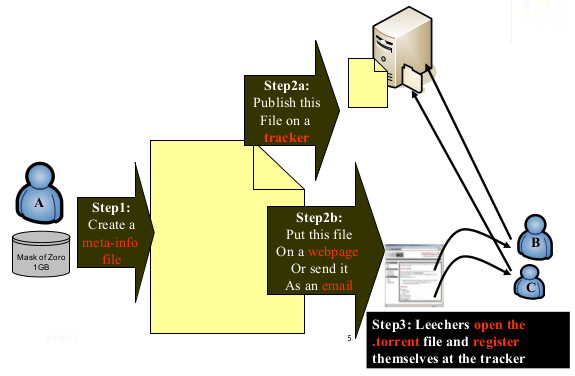
\includegraphics[width=7cm]{img/torrent.png}
\item[Handshaking]: Once a peer list is received, a handshake message
is sent to the all peers
\item[Exchanging bitfields] after handshaking with peers

\end{description}

\begin{figure}[!ht]
\centering
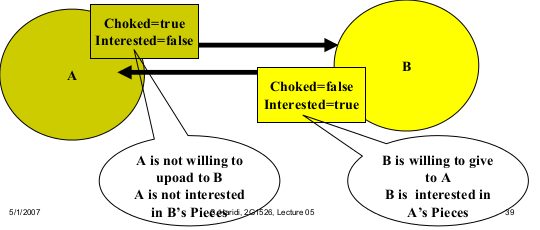
\includegraphics[width=9cm]{img/after.png}
\caption{After exchange}
\end{figure}
\FloatBarrier{}

%TODO Choking

\subsubsection{Piece selection}
\begin{itemize}
\item Rarest-first amoung your peers
\item Random-first piece to get first piece as fast as possible (only first few piece)
\item EndGame mode
\end{itemize}

\subsubsection{Peer selection}
\begin{enumerate}
\item Construction of the peer list by using the tracker
\item Unchoking (=Choice based on which peer can give me pieces faster)

\begin{itemize}
    \item A peer has a total of 80 connections, 40 initiated by
    him and 40 by others
    \item A peer unchokes only 4 peers simultaneously
    \item Decision about unchoking is reconsidered every ten
    seconds
    \begin{itemize}
        \item 3 peers are unchoked (given that they are interested)
        based on their upload rate to me
        \item Optimistically look for a fast guy randomly in the 40
        remaining connections
    \end{itemize}
\end{itemize}
\end{enumerate}
